\documentclass[a4paper, 11pt]{article}

\usepackage{adjustbox}
\usepackage{amsmath}
\usepackage{amssymb}
\usepackage{booktabs}
\usepackage{caption}
\usepackage[labelfont=bf,font=footnotesize]{caption}
\usepackage{dirtytalk}
\usepackage[symbol]{footmisc}
\usepackage{geometry}
\usepackage{graphicx}
% \usepackage{natbib}
\usepackage{parskip}
\usepackage{physics}
\usepackage[obeyspaces]{xurl}
\usepackage{siunitx}
\usepackage{calc}

\usepackage[dvipsnames,table]{xcolor}
\usepackage{textcomp}

\usepackage[hypertexnames=false,hidelinks]{hyperref}
\usepackage[noabbrev,nameinlink,capitalize,poorman]{cleveref}

% \setcitestyle{square}
\bibliographystyle{plain}

\begin{document}
\begin{titlepage}
    \begin{minipage}{0.5\textwidth}
        \vspace{-2cm}
        \hspace{-1cm}
        
\includegraphics[width=1\textwidth]{uni_logo.jpg}
    \end{minipage}
    \begin{center}
        \vspace{6cm}
        \begin{minipage}{0.7\textwidth}
        \centering
        {\huge\bfseries Coursework \vspace{10pt}\\ Deep Learning for Sequence Analysis  \vspace{10pt} \\ INM706}\\[2ex]
        \vspace{15pt}
        {\LARGE Alessandro Abati \& Martin Fixman}\\[1ex]
        {\large student IDs: 230040125 \& 230053494}\\[1ex]
        {\Large \today}
        \end{minipage}
    \end{center}
    \begin{center}
        {\Large \href{https://github.com/mfixman/ai-sequential}{GitHub repository}}
    \end{center}
\end{titlepage}

\clearpage{}
\thispagestyle{empty}
\tableofcontents

\clearpage{}
\section{Introduction}
Abstractive text summarization is a complex and evolving field in natural language processing (NLP) that focuses on generating concise and coherent summaries from longer text documents. Unlike extractive summarization, which involves selecting and concatenating sentences directly from the source text, abstractive summarization aims to produce a summary that captures the essence of the original content in a new, rewritten form. This involves the model understanding the context and generating novel phrases, often utilizing vocabulary not present in the source document.

The task of abstractive summarization poses several challenges. One of the primary difficulties is ensuring that the generated summary is both coherent and relevant to the main points of the source text. Additionally, the model must handle issues such as maintaining grammatical correctness and avoiding redundancy, which are crucial for producing high-quality summaries.

Recent advancements in deep learning have significantly improved the performance of abstractive summarization models. Sequence-to-sequence (Seq2Seq) models, particularly those incorporating attention mechanisms, have become the standard approach for this task. The attentional encoder-decoder model \cite{bahdanau2014neural} introduced the concept of allowing the model to focus on different parts of the input sequence while generating each word of the output sequence.

Following this, several improvements and variations have been developed such as a model where the decoder was replaced with an RNN \cite{Chopra2016AbstractiveSS}. 

In addition to RNN-based models, transformer-based architectures have also been explored extensively. Transformer model \cite{transformer} relies on self-attention mechanisms to process the entire input sequence simultaneously, offering better parallelization and efficiency during training. Subsequent models like BERT \cite{devlin2018bert} and GPT-2 \cite{radford2019language} have been adapted for summarization tasks, leveraging their pre-training on large corpora to improve performance in low-data settings.

The primary objective of this research is to develop and evaluate different neural network architectures for abstractive text summarization, focusing on enhancing model performance through various techniques. Our methodology includes the implementation of Seq2Seq models with attention mechanisms, transformer models, and hybrid approaches that combine pre-trained models like BERT and GPT-2 with custom encoder-decoder architectures. We employ the CNN/Daily Mail dataset, a well-known benchmark in the field, to train and test our models. The dataset contains news articles and their corresponding highlights, which serve as the ground truth summaries. We utilized the 3.0.0 version of the dataset from the \textit{Hugging Face} datasets library \cite{huggingface_cnn_dailymail}.



\clearpage{}
\section{Methodology}

\subsection{Data preprocessing}

\subsubsection{Tokenisation}
For processing the data must be separated into tokens, which are later one-hot-encoded into the models (which include the embeddings).

This tokenisation is not trivial, since having too many words can unnecessarily produce high dimensionality in the embeddings which can make the model slower and more efficient.
To prevent this we use a pretrained BERT subword tokeniser\cite{BERTtokenizer}.

\begin{figure}[h]
	\newcommand{\hh}{\texttt{\#\#}}
	\newcommand{\tokbox}[1]{\fbox{\strut\centering #1}}
	\centering
	\fbox{\parbox{\textwidth}{\fbox{\parbox{\textwidth - 13pt}{\small\sffamily the head of pakistan's ruling coalition announced thursday that the government will \\ move to impeach president pervez musharraf}}}} \\
	\fbox{\parbox[m][][t]{\textwidth}{\small \sffamily
		 \tokbox{the}%
		 \tokbox{head}%
		 \tokbox{of}%
		 \tokbox{pakistan}%
		 \tokbox{'}%
		 \tokbox{s}%
		 \tokbox{ruling}%
		 \tokbox{coalition}%
		 \tokbox{announced}%
		 \tokbox{thursday}%
		 \tokbox{that}%
		 \tokbox{the}%
		 \tokbox{government}%
		 \tokbox{will}
		 \tokbox{move}%
		 \tokbox{to}%
		 \tokbox{imp}%
		 \tokbox{\hh{}ea}%
		 \tokbox{\hh{}ch}%
		 \tokbox{president}%
		 \tokbox{per}%
		 \tokbox{\hh{}vez}%
		 \tokbox{mu}%
		 \tokbox{\hh{}sha}%
		 \tokbox{\hh{}rra}%
		 \tokbox{\hh{}f}
	 }}
	\caption{Example of BERT tokeniser. Long words not in the dictionary, such as \textsf{``musharraf''}, get converted into several tokens that can be shared between words.}
\end{figure}

Each one of these tokens (including special tokens such as \texttt{<SOS>}) is transformer to a single integer from 0 to \num{30522}.
The embedding layer, present in all our models, returns a spatial embedding.

\subsubsection{Punctuation}
Most punctuation is removed from the dataset, as it doesn't help in our objective of summarising a text.
Periods \textsf{`\textbf{.}'} are retained, since they help separate between the many news in our input text.
We also do not delete apostrophes \textsf{`\textbf{'}'}, as they are an integral part of the English language\cite{apostrophes}.

\subsubsection{TF and IDF Metrics Embedding}

All of our enhanced models compute Term Frequency (TF) and Inverse Document Frequency (IDF) metrics for the dataset\cite{nallapati2016abstractive}.
These metrics measure how frequently a term occurs in a document, and how important this term is respectively.
\begin{align}
	\text{TF}(t) &= \frac{\text{Number of times term $t$ appears in a document}}{\text{Total number of terms in the document}} \\[1ex]
	\text{IDF}(t) &= \log \left( \frac{\text{Total number of documents}}{\text{Number of documents with term $t$ in it}} \right)
\end{align}

The inclusion of these embeddings aimed to provide the model with additional information about the importance of words in the context of the entire dataset, potentially improving the quality of the generated summaries.

\subsection{Loss Function(s)}

\subsubsection{Categorical Cross-Entropy Loss}

Part of our loss function is the Categorical Cross-Entropy Loss\cite{cross_entropy_loss}, which achieves a smooth gradient function by calculating the loss with the logits of the result rather than the result itself.
\begin{equation}
	\mathcal{L}_\text{CCE} = - \frac{1}{N} \frac{1}{W} \sum_{n=1}^{N} \sum^W_{w = 1} \log(p_{n,w,y_{n,w}})
\end{equation}

This loss is calculated separately between each pair of words between the prediction and the target set, where it's averaged between all words and all batches.
While it does predict how close the prediction is to exact value of the target, it does not separate between a slightly different and a completely unrelated word.

\subsubsection{Cosine Similarity Loss}
\label{cosine_similarity_loss}

We can use the embeddings to estimate how close each predicted word to the real target\cite{cosineSimilarity}.
\begin{equation}
	\mathcal{L}_\text{CS} = 1 - \frac{1}{N} \sum_{n=1}^{N} \sum^W_{w = 1} \frac{\mathbf{x}_{n,w} \cdot \mathbf{y}_{n,w}}{\|\mathbf{x}_{n,w}\| \|\mathbf{y}_{n, w}\|}	
\end{equation}

This loss function would help us reach a result that's meaningful rather than identical to the target, as in the CCE loss.

However, when training embeddings as part of a larger model, relying solely on cosine similarity loss can be problematic since the loss is minimized when the embeddings of all words become very close to each other.
This reduces the ability of the embeddings to capture distinct and meaningful differences between words, which might collapse of embeddings into a small region of the space can lead to poor generalization and a lack of discrimination between different words.

\subsection{Combined Cross Similarity}
We introduce \emph{Combined Cross Similarity Loss}, which combines both CCE and CS losses into a single category in a way that's controlled by a parameter $\varkappa$.
\begin{equation}
    \mathcal{L} = (1 - \varkappa) \mathcal{L}_{\text{CCE}} + \varkappa \mathcal{L}_{\text{CS}}
\end{equation}

A higher $\varkappa$ gives more weight to the cosine-similarity loss component of the loss, while a lower one gives more weight to the categorical cross-entropy component.
The ideal value, along with other components, will be found in a parameter sweep.

Unfortunately, the section in \cref{param_sweep_section} showed that having $\varkappa = 0$ produces a better result for low learning rate.
This probably speaks of the strength of categorical cross-entropy as a loss.

\subsection{Scoring Functions}
\label{scoring_section}
\subsubsection{ROUGE-1 and ROUGE-2}
To evaluate the performance of our models, we utilized the ROUGE (Recall-Oriented Understudy for Gisting Evaluation) metrics, which are the standard benchmark for abstractive text summarization tasks\cite{abstCNN}.

Specifically, we calculated the ROUGE-1 and ROUGE-2 scores, which measure the overlap of unigrams and bigrams between the generated summaries and the reference summaries, respectively. These scores are calculated based on precision, recall, and F1-score:
\begin{equation}
    \begin{split}
        &\text{Precision}_{\text{ROUGE-N}} = \frac{|\text{n-grams}_{\text{Prediction}} \cap \text{n-grams}_{\text{Target}}|}{|\text{n-grams}_{\text{Prediction}}|}
        \\\\
        &\text{Recall}_{\text{ROUGE-N}} = \frac{|\text{n-grams}_{\text{Prediction}} \cap \text{n-grams}_{\text{Target}}|}{|\text{n-grams}_{\text{Target}}|}
        \\\\
        &\text{ROUGE-N} = \text{F1}_{\text{ROUGE-N}} = \frac{2 \cdot \text{Precision}_{\text{ROUGE-N}} \cdot \text{Recall}_{\text{ROUGE-N}}}{\text{Precision}_{\text{ROUGE-N}} + \text{Recall}_{\text{ROUGE-N}}}
    \end{split}
\end{equation}

In contrast to typical ROUGE implementations, which take text as input and tokenize it internally, we developed a custom approach to calculate the ROUGE metrics directly on the token indices.
This method ensures that the evaluation is consistent with the tokenization scheme used during model training and inference, and that the results can be found quickly using GPU processing.

\subsubsection{Cosine Similarity Score}
In addition to the cosine similarity loss used in \cref{cosine_similarity_loss}, we use the cosine similarity as a scoring and comparing models.


\section{Models}
\label{models_section}
\subsection{Baseline Model: Seq2Seq}

We initially implemented a Seq2Seq model\cite{sutskever2014sequence} using an encoder-decoder architecture with Long Short-Term Memory (LSTM) layers\cite{lstm}.

The Seq2Seq model processes an input sequence and generates an output sequence, predicting one token at a time in an autoregressive manner. The general functioning of the Seq2Seq model can be described as follows:

\paragraph{Encoder:}
The encoder takes an input sequence \( X = (x_1, x_2, \ldots, x_n) \) and processes it through multiple LSTM layers to produce a set of hidden states \( \mathbf{H} = (\mathbf{h}_1, \mathbf{h}_2, \ldots, \mathbf{h}_n) \). Before the LSTM layers, an embedding layer is used to convert the input tokens into dense vectors of a fixed size. The final hidden state and cell state of the encoder are passed to all the layers of the decoder as the initial states. The encoder's operations can be expressed as:
\begin{equation}
    \mathbf{e}_t = \text{Embedding}(x_t) \,\, \rightarrow \,\, \mathbf{h}_t = \text{LSTM}(\mathbf{e}_t, \mathbf{h}_{t-1})
\end{equation}
where \( \mathbf{e}_t \) is the embedding of the input token \( x_t \) and \( \mathbf{h}_t \) is the hidden state at time step \( t \).

\paragraph{Decoder:}
The decoder generates the output sequence \( Y = (y_1, y_2, \ldots, y_m) \) one token at a time. At each time step \( t \), the decoder takes the previous token \( y_{t-1} \), the previous hidden state, and the previous cell state as inputs, and produces the current token \( y_t \). An embedding layer is also used in the decoder to convert the input tokens into dense vectors before passing them to the LSTM layers. Initially, the decoder receives the start-of-sequence token \( \langle \text{sos} \rangle \) as the first input. The decoder's operations can be described as:
\begin{equation}
    \mathbf{e}_t' = \text{Embedding}(y_{t-1}) \,\, \rightarrow \,\, \mathbf{h}_t = \text{LSTM}(\mathbf{e}_t', \mathbf{h}_{t-1})
\end{equation}
where \( \mathbf{e}_t' \) is the embedding of the previous output token \( y_{t-1} \), \( \mathbf{h}_t \) is the hidden state at time step \( t \).

\subsubsection{Bahdanau Attention}

As an improvement to the basic Seq2Seq model, we incorporated Bahdanau Attention\cite{bahdanau2014neural} only in the decoder. This attention mechanism allows the model to focus on relevant parts of the input sequence at each decoding step, improving the quality of the generated summaries.

The Bahdanau attention weights can be formulated as:
\begin{equation}
    \alpha_{t,i} = \frac{\exp(e_{t,i})}{\sum_{j=1}^{T} \exp(e_{t,j})}
\end{equation}
where \( e_{t,i}\) are the attention scores based on the alignment between the decoder's hidden state and the encoder's output states:
\begin{equation}
    e_{t,i} = \mathbf{v}^T \tanh(\mathbf{W}_a \mathbf{h}_t + \mathbf{U}_a \mathbf{h}_i)
\end{equation}
where \( \mathbf{h}_t \) is the decoder's hidden state at time step \( t \), \( \mathbf{H} = \{\mathbf{h}_1, \mathbf{h}_2, \ldots, \mathbf{h}_T\} \) is the encoder's outputs, \( \mathbf{W}_a \) and \( \mathbf{U}_a \) are learnable weight matrices, and \( \mathbf{v} \) is a learnable parameter vector.
The output of the attention layer is:
\begin{equation}
    \mathbf{h}'_t = \tanh(\mathbf{W}_c [\mathbf{c}_t ; \mathbf{h}_t])
\end{equation}
where \( \mathbf{W}_c \) is a learnable weight matrix and \( [\mathbf{c}_t ; \mathbf{h}_t] \) denotes the concatenation of the decoder's hidden state and the context vector:
\begin{equation}
    \mathbf{c}_t = \sum_{i=1}^{T} \alpha_{t,i} \mathbf{h}_i
\end{equation}

The decoder uses this context vector \( \mathbf{c}_t \) along with its hidden states to generate the output tokens. This mechanism enhances the model's ability to focus on the most relevant parts of the input sequence during each step of the decoding process.

The Seq2Seq model with Bahdanau attention was trained using top-10 sampling and teacher forcing with an initial ratio of 0.5, which decreased by 0.0005 at every step. The teacher forcing ratio allows the model to gradually learn to generate sequences independently by reducing the dependency on the correct previous token over time.

\subsection{Transformer Model}

The Transformer model\cite{vaswani2017attention}, implemented using PyTorch's \textit{nn.Transformer} class\cite{transformer}, is another architecture usually employed for abstractive text summarization. Unlike the Seq2Seq model, the Transformer relies on self-attention mechanisms to process the entire input sequence simultaneously, allowing for more parallelization and efficient training.

\subsubsection{Self-Attention Mechanism}

The self-attention mechanism is a key component of the Transformer model, allowing the model to weigh the importance of different tokens in the input sequence dynamically. The attention mechanism operates as follows:

Given an input sequence \(\mathbf{X} \in \mathbb{R}^{n \times d}\), where \(n\) is the sequence length and \(d\) is the embedding dimension, we compute the Query (\(\mathbf{Q}\)), Key (\(\mathbf{K}\)), and Value (\(\mathbf{V}\)) matrices as:
\begin{equation}
     \mathbf{Q} = \mathbf{X}\mathbf{W^Q}, \quad \mathbf{K} = \mathbf{XW^K}, \quad \mathbf{V} = \mathbf{XW^V}
\end{equation}
where \(\mathbf{W^Q}, \mathbf{W^K}, \mathbf{W^V} \in \mathbb{R}^{d \times d_k}\) are learnable weight matrices.

The attention scores are computed as:
\begin{equation}
    \text{Attention}(\mathbf{Q}, \mathbf{K}, \mathbf{V}) = \text{softmax}\left(\frac{\mathbf{Q}\mathbf{K}^T}{\sqrt{d_k}}\right)\mathbf{V}
\end{equation}
where \(d_k\) is the dimensionality of the queries and keys.

Multi-head attention extends this by allowing the model to jointly attend to information from different representation subspaces at different positions. This is achieved by concatenating the outputs of \(h\) attention heads:
\begin{equation}
    \text{MultiHead}(\mathbf{Q}, \mathbf{K}, \mathbf{V}) = \text{Concat}(\text{head}_1, \ldots, \text{head}_h)\mathbf{W^O}
\end{equation}
where \(\text{head}_i = \text{Attention}(\mathbf{Q}\mathbf{W^Q}_i, \mathbf{K}\mathbf{W^K}_i, \mathbf{V}\mathbf{W^V}_i)\), and \(\mathbf{W^O} \in \mathbb{R}^{hd_k \times d}\).

\subsubsection{Positional Encoding and Masking}

Since the Transformer model lacks recurrence, it does not have a built-in sense of the order of words in a sequence. To address this, positional encodings are added to the input embeddings to provide information about the position of each token within the sequence.

The positional encoding for a position \(pos\) and dimension \(i\) is defined as:
\begin{equation}
	\begin{aligned}
		PE_{(pos, 2i)} &= \sin\left(\frac{pos}{10000^{2i/d}}\right) \\
		PE_{(pos, 2i+1)} &= \cos\left(\frac{pos}{10000^{2i/d}}\right)
	\end{aligned}
\end{equation}
where \(d\) is the dimensionality of the embeddings. These positional encodings are added to the input embeddings to inject positional information.

Masking is also crucial in the Transformer architecture. We employed two types of masks: a padding mask to prevent the model from attending to padding tokens in the input and a target sequence mask to ensure that the model only attends to previous tokens in the target sequence during training.


\subsection{BERTformer}
Bidirectional Encoder Representations from Transformers (BERT)\cite{devlin2018bert} is a language model designed to understand the context of words in a sentence by considering both the left and right surroundings (bidirectional context).
Unlike traditional left-to-right or right-to-left training, BERT is trained on masked language modeling (MLM) and next sentence prediction (NSP) tasks, enabling it to capture a deep understanding of language nuances and context.

In our approach, we implemented a custom transformer model, named BERTformer, by combining the pre-trained frozen BERT model as the encoder and the standard Transformer decoder from the PyTorch \textit{nn.Transformer} library.
This hybrid architecture aims to leverage BERT's robust embeddings effectively capture the meaning and context of news articles, thus facilitating better summarization.

The encoder component of BERTformer utilizes the BERT-base model from HuggingFace \cite{BERTHugginFace}, which consists of 12 transformer layers with 768 hidden units and 12 self-attention heads.
The BERT encoder had been fed with the embedded masked input sequences, including positional embedding, TF and IDF metrics.
The input sequence had to be truncated to a maximum size of 512 tokens.
The output of the BERT encoder, which consists of contextualized embeddings, is passed to the transformer decoder, which is the decoder class of the Pytorch's implementation.


\clearpage{}
\section{Parameter Sweep}
\label{param_sweep_section}

In order to find the parameters for the two enhanced models that maximise some of our scores, we run a full parameter sweep on a subset of the samples with two parameters related to training.
\begin{table}[h]
	\centering
	\begin{tabular}{r | l l l}
		\toprule
			Parameter & \multicolumn{3}{|c}{Values} \\
		\midrule
			Learning Rate ($\alpha$) & 0.01 & 0.001 & 0.0001 \\
			Cosine Similarity Weight ($\varkappa$) & 0 & 0.2 & 0.5 \\
		\bottomrule
	\end{tabular}
\end{table}

Each model is run for 15 epochs, since in our experiments that's enough for finding a trend in the metrics, and is judged in three of the metrics presented in \cref{scoring_section}: F1-score of Rouge1, F1-score of Rouge2, and cosine similarity score.

\subsection{Transformer Model}

The results can be found in the three scatter plots in \cref{sweep_results}.
\begin{figure}[h]
	\centering
	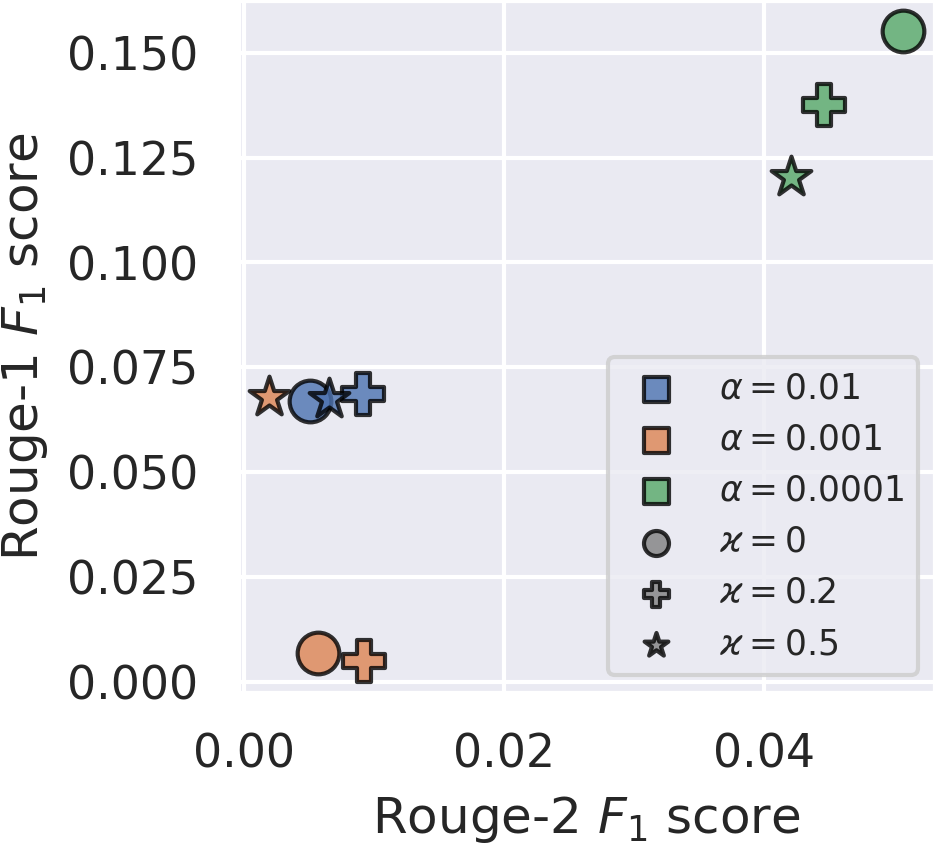
\includegraphics[width=.32\textwidth]{sweep_rouge1_v_rouge2.png} \hfill{}
	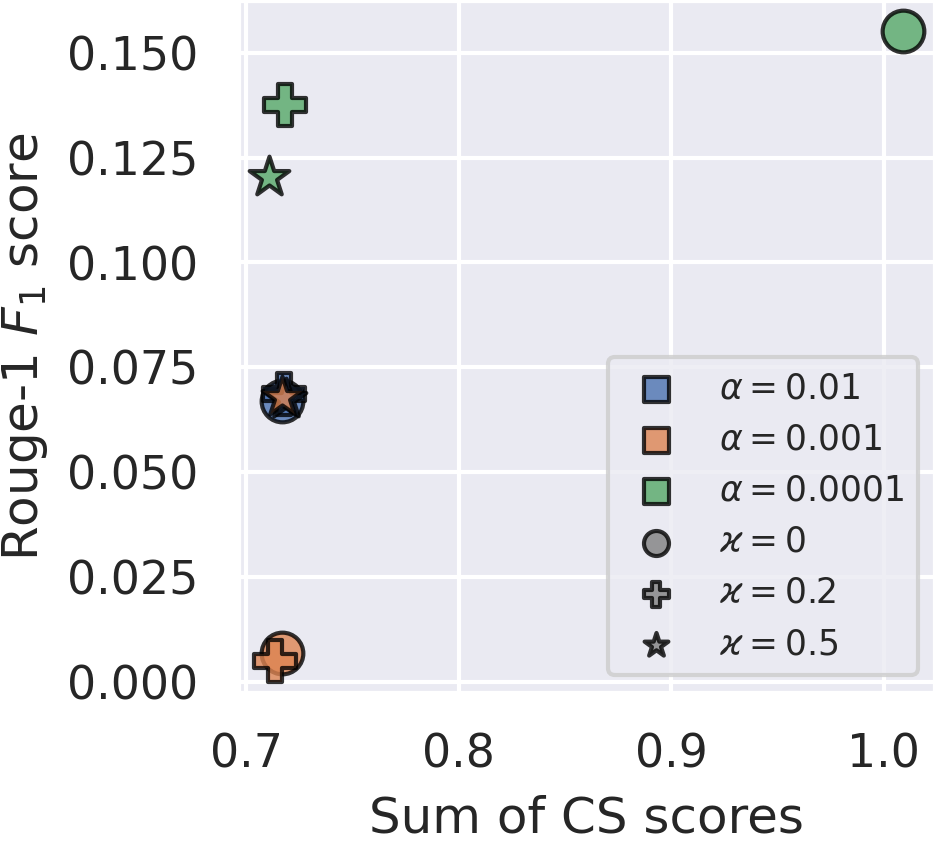
\includegraphics[width=.32\textwidth]{sweep_rouge1_v_cs.png} \hfill{}
	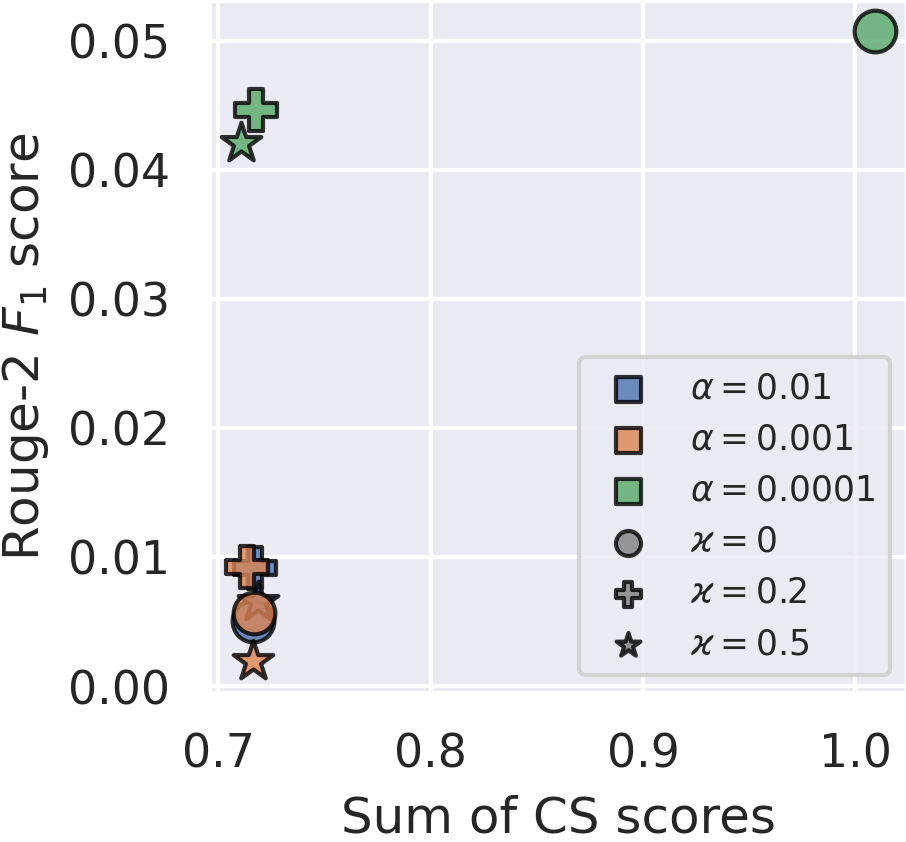
\includegraphics[width=.32\textwidth]{sweep_rouge2_v_cs.png}
	\caption{Results of parameter sweep of the transformer for different $\alpha$ and $\varkappa$ values. For all three scores, $\alpha = 0.0001$ and $\varkappa = 0$ presents the best results.}
	\label{sweep_results}
\end{figure}

The main results from the parameter sweep clearly demonstrate that, in the case of this transformer, a low learning rate produces better results in all metrics that a high learning rate.
This is a bit surprising given the large amount of parameters the transformer, but it's likely related to how unstable problem in sequence analysis are: even a small change in weights produces a large change in these metrics, so convergence must be slower.

Additionally, it's sadly clear that the best result at this learning rate happen when $\varkappa = 0$.
While using cosine similarity loss as a fraction of the final loss seemed like a fine idea, it's likely that it adds extra instability to the gradient descent.

\newpage{}
\subsection{BERTFormer}

The results from the parameter sweep can be found in the three scatter plots in \cref{bertformer_sweep_results}.

\begin{figure}[h]
	\centering
	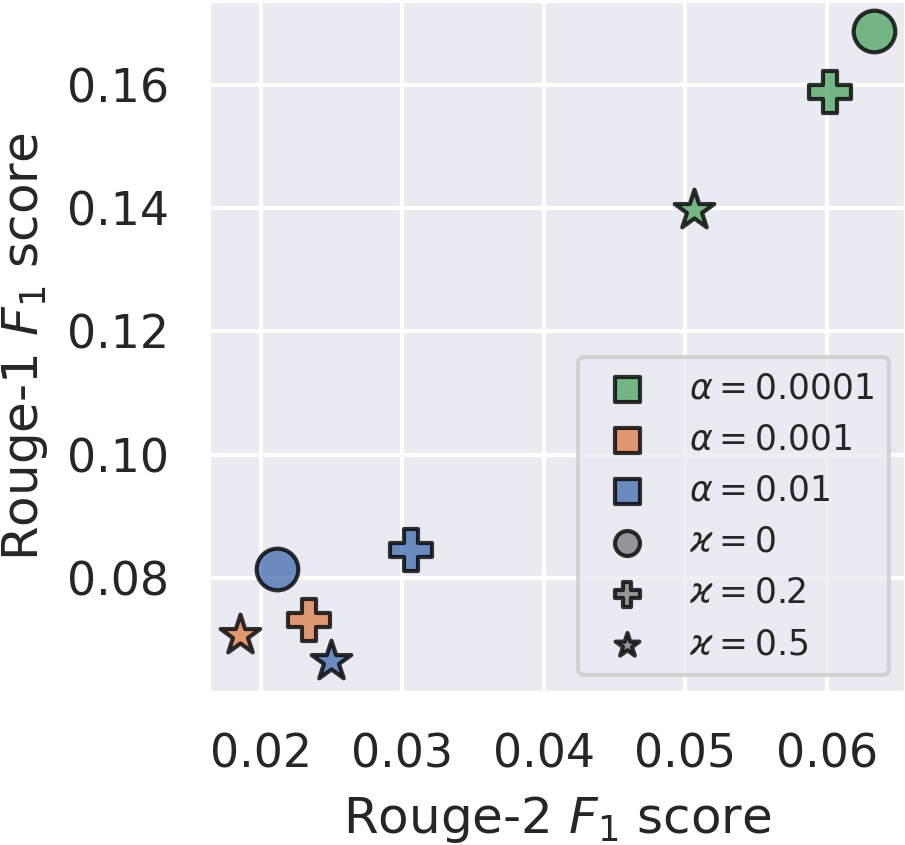
\includegraphics[width=.32\textwidth]{bertformer_sweep_rouge1_v_rouge2.png} \hfill{}
	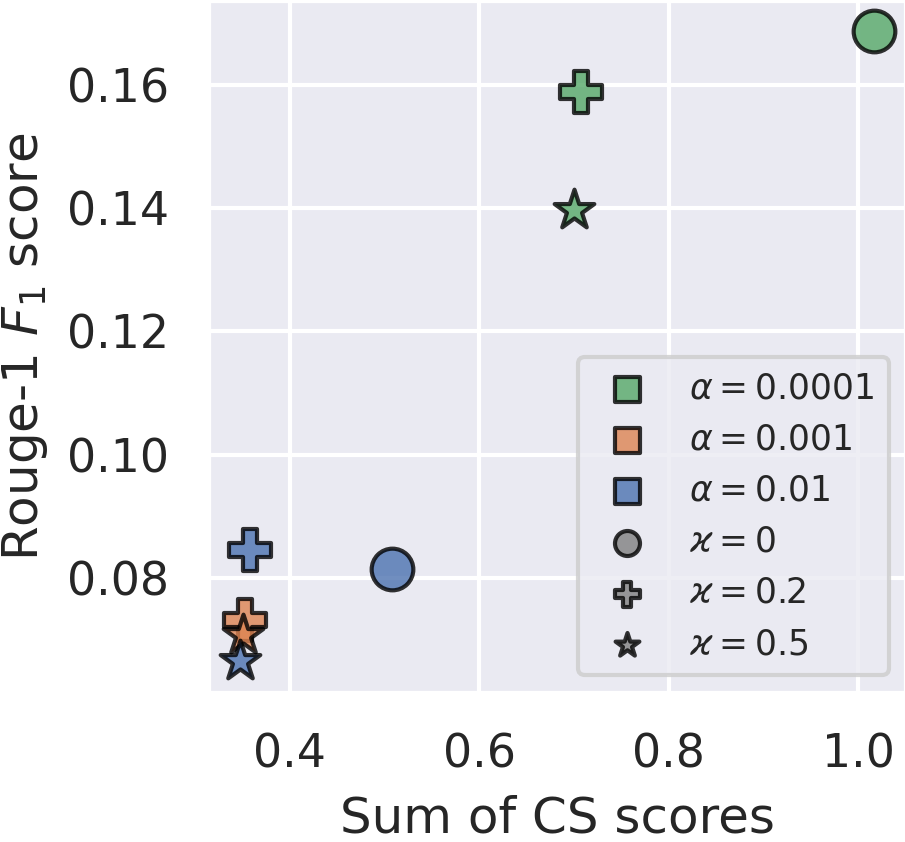
\includegraphics[width=.32\textwidth]{bertformer_sweep_rouge1_v_cs.png} \hfill{}
	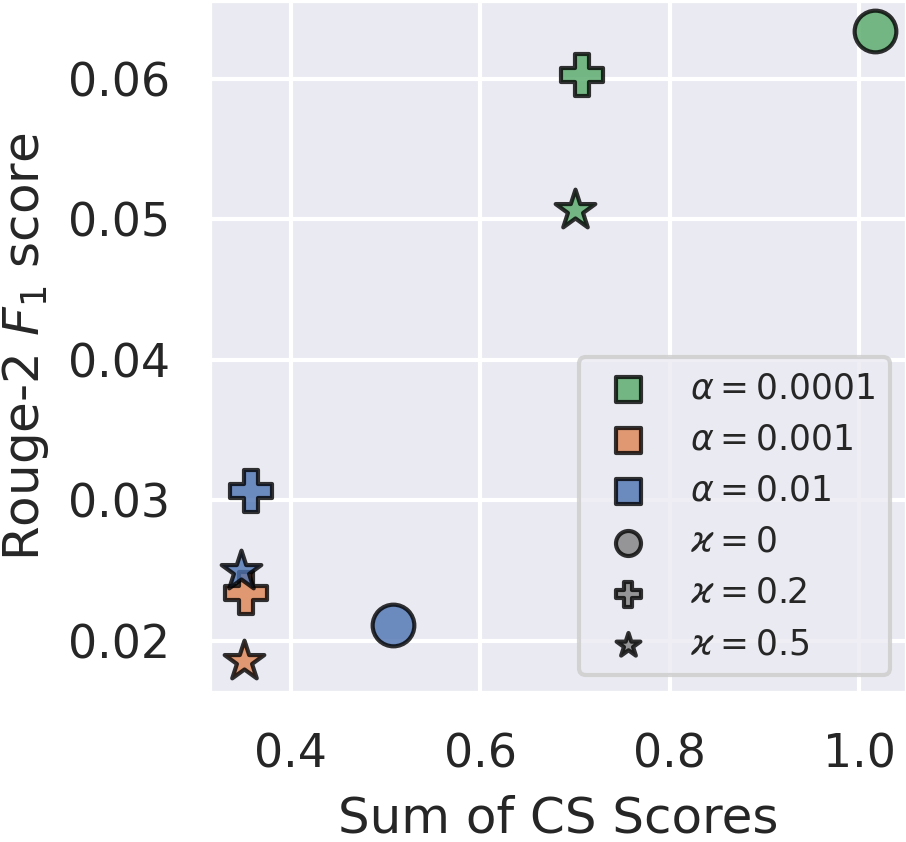
\includegraphics[width=.32\textwidth]{bertformer_sweep_rouge2_v_cs.png}
	\caption{Results of parameter sweep of the transformer for different $\alpha$ and $\varkappa$ values. For all three scores, $\alpha = 0.0001$ and $\varkappa = 0$ presents the best results.}
	\label{bertformer_sweep_results}
	\vspace{-7pt}
\end{figure}

The results are very similar to those in \cref{sweep_results}, and both parameter sweeps have a clear winner with low learning rate and no use of cosine similarity loss ($\varpappa = 0$).

Despite this, the BERTFormer models using $\varkappa > 0$ seems to have better results on CS score than the Transformer model when trained on the small amount of samples that were needed for a run in this parameter sweep.
This is likely due to the pre-trained encoder producing more sensible language without need for much training, and is worth experiment on in the future.

\subsection{Final Results}

\begin{table}[h]
	\centering
	\begin{tabular}{l c | c c | c c c}
		\toprule
			Model & Best & $\alpha$ & $\varkappa$ & Rouge-1 $F_1$ & Rouge-2 $F_1$ & Sum of CS \\
		\midrule
			Transformer & 
\includegraphics[width=9pt,height=9pt]{green_circle.png} & 0.0001 & 0 & 0.17 & 0.69 & 1.02 \\
			BERTFormer & 
\includegraphics[width=9pt,height=9pt]{green_circle.png} & 0.0001 & 0 & 0.16 & 0.62 & 1.01 \\
		\bottomrule
	\end{tabular}
	\caption{The models with the best scores in the hyperparameter, which contains the parameters we will use for them from now on.}
\end{table}



\clearpage{}
\section{Results}

\subsection{Seq2Seq and Transformer models}
Both the Seq2Seq and Transformer models seem to train slowly due to the large amount of data provided.

While we were not able to train many epochs due to technical reasons, this didn't seem to be necessary as both models have a minimal loss at epochs 11 and 14, respectively.

\begin{figure}[h]
	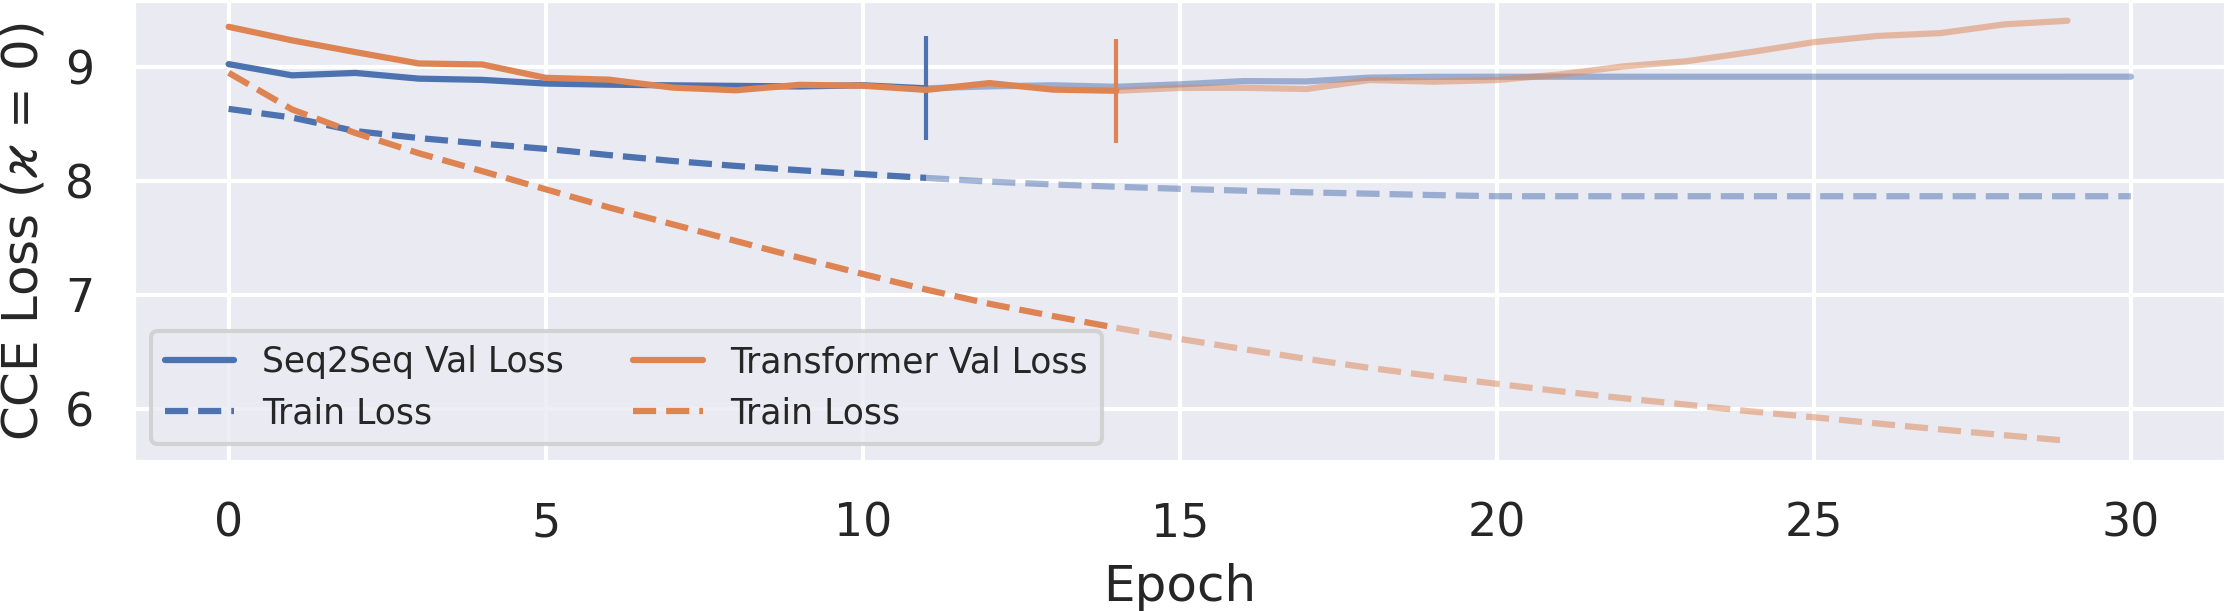
\includegraphics[width = \textwidth]{baseline_losses.png}
	\caption{Training and validation losses of both initial models. Due to early stopping, only the non-transparent part is considered.}
\end{figure}

While the categorical cross-entropy loss of these models seems similar, their ROUGE scores tell another story.
\Cref{baseline_rouges} contains the ROUGE1 and ROUGE2 scores of both models, where the transformer produces a considerably better score.

\begin{figure}[h]
	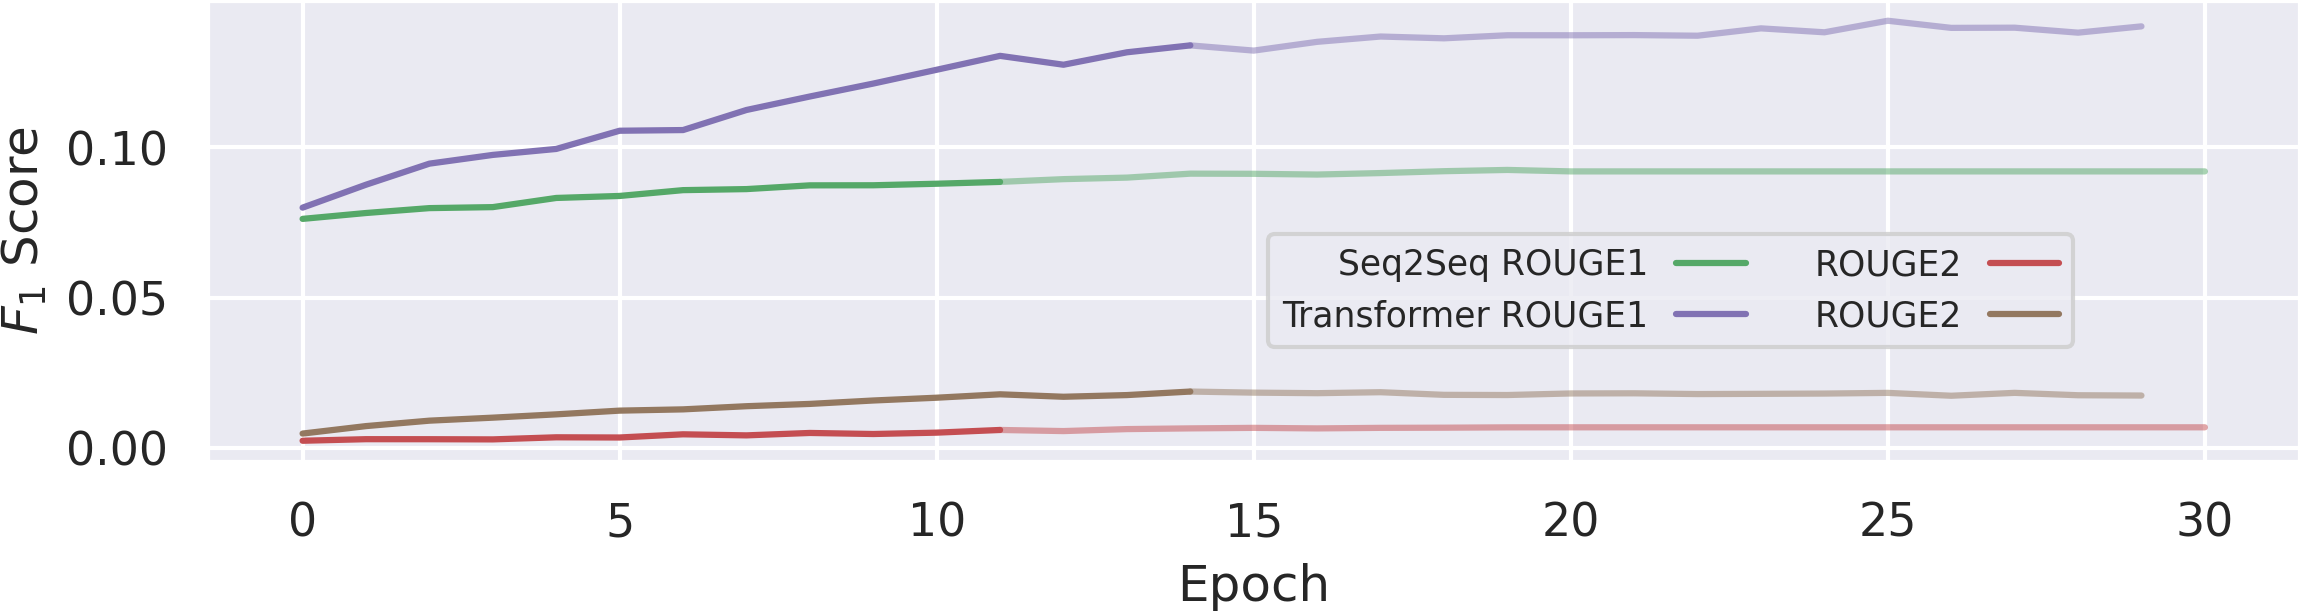
\includegraphics[width = \textwidth]{baseline_rouges.png}
	\caption{ROUGE scores of the Seq2Seq and Transformer models. The attention mechanism allows the transformer model to create more coherent result with higher ROUGE scores.}
	\label{baseline_rouges}
\end{figure}

Are these relatively good ROUGE scores good for having reasonable results?
The answer is a resounding \textbf{NO}.

\Cref{seq2seq_example,transformer_example} in \appendixA show some examples of the outputs from this model.
The results are nonsensical, and there is nothing that could even suggest where to start.


\clearpage{}
\section{Conclusions}
\paragraph{COmment To be changed!}Fine.tuning BERT and GPT models could help improving teh performance by adapting teh mdoels to the abstarctive text sumamrization task - This requires a lot of computational resources and time!!!

\section{Reflections}
\paragraph{Period (".") token}
During our experimentation, we observed that omitting the period (".") token from the model resulted in significant confusion in the source news, as it failed to distinguish between sentences effectively. This issue was evident in the summaries, where unrelated tokens often appeared consecutively.

Consequently, we decided to include the period (".") token in our dataset to better delineate sentences within the sequences. This inclusion aims to improve the clarity and coherence of the generated summaries. However, this approach has a potential drawback, as the period token becomes disproportionately important throughout the dataset, particularly influencing Term Frequency (TF) and Inverse Document Frequency (IDF) metrics.

For future work, we recommend that the TF and IDF metrics should not be calculated for the period token. Alternatively, the end-of-sequence token could be employed to mark sentence boundaries, which might offer a more effective solution.

\paragraph{NER embedding}
An important future direction for enhancing our model involves the integration of a Named Entity Recognition (NER) model in the preprocessing step of the dataset. The NER model would extract information about the entities present in the dataset, which would then be embedded alongside the contextual output of the encoder. This additional layer of information aims to provide the model with a deeper understanding of the entities involved in the news articles, potentially improving the accuracy and relevance of the generated summaries. 

Specifically, we plan to utilize the pre-trained BERT-base-NER model\cite{BERTNER}, which has been trained to recognize four types of entities: locations (LOC), organizations (ORG), persons (PER), and miscellaneous entities (MISC). 



\clearpage{}

\bibliography{sequential_report.bib}

\end{document}

